\title{Singular Vectors}
\subtitle{\SubTitleName}
\institute[]{\Course}
\author{\Instructor}
\maketitle   


\frame{\frametitle{Topics and Objectives}
\Emph{Topics} \\
%\TopicStatement
\begin{itemize}

    \item singular vectors (the eigenvectors of $A^TA$)

\end{itemize}

\vspace{0.5cm}

\Emph{Learning Objectives}\\

%\LearningObjectiveStatement

\begin{itemize}
    \item apply the eigenvectors of $A^TA$ to construct a basis for $\Col A$, $\Row A$, and $\Nul A$
    \item determine the rank of a matrix using the singular values of that matrix
\end{itemize}

} 

\begin{frame}{Motivation: The Four Fundamental Subspaces}

    \begin{center}\begin{tikzpicture} \node [mybox](box){\begin{minipage}{0.85\textwidth}\vspace{2pt}
    For any $ A \in \mathbb R^{m\times n}$,  the orthogonal complement of $\Row A$ is $ \Null A$, and the orthogonal complement of $ \Col A$ is  $ \Null A ^{T}$.  

    \end{minipage}};
    \node[fancytitle, right=10pt] at (box.north west) {Theorem (The Four Subspaces)};
    \end{tikzpicture}\end{center}

    % The idea behind this theorem is described in the diagram below. 
    \pause 
    
    \begin{center}
    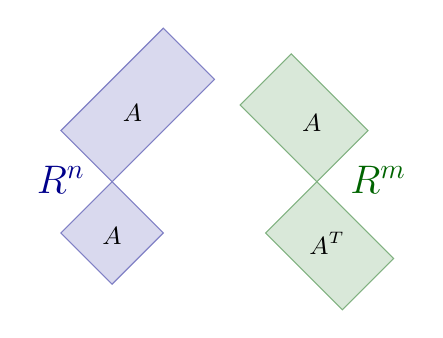
\begin{tikzpicture}[scale=.65]
        
        \onslide<2->{
        % boxes
        \filldraw[draw=DarkBlue!50,fill=DarkBlue!15] (0,0) -- (-1,1) -- (1,3) -- (2,2) -- cycle;
        \filldraw[draw=DarkBlue!50,fill=DarkBlue!15] (0,0) -- (1,-1) -- (0,-2) -- (-1,-1) -- cycle;      
        \draw (0.4, 1.7) node[below]{\small $\Row A$};
        \draw (0.0,-0.7) node[below]{\small $\Nul A$};        
        }
        
        \onslide<3->
        {
        \filldraw[draw=DarkGreen!50,fill=DarkGreen!15] (4,0) -- (2.5, 1.5) -- (3.5, 2.5) -- (5,1) -- cycle;
        \filldraw[draw=DarkGreen!50,fill=DarkGreen!15] (4,0) -- (5.5,-1.5) -- (4.5,-2.5) -- (3,-1) -- cycle;        
        \draw (3.9, 1.5) node[below]{\small $\Col A$};
        \draw (4.2, -0.8) node[below]{\small $\Nul A^T$};        
        }

        \onslide<4->{
        \draw (-1.0,0.5) node[below]{\Large $\color{DarkBlue} \mathbb R^n$};
        }

        \onslide<5->{
        \draw ( 5.2,0.5) node[below]{\Large $\color{DarkGreen} \mathbb R^m$};
        }
        
    \end{tikzpicture}
    \end{center}
    \pause 
    The eigenvectors of $A^TA$ can be used construct bases for these subspaces. 
\end{frame}

\begin{frame}\frametitle{Orthogonal Bases for $\Nul A$ and $\Row A$}

    \begin{center}\begin{tikzpicture} \node [mybox](box){\begin{minipage}{0.94\textwidth}\vspace{2pt}
        
        Suppose $\vec v_i$ are the $n$ orthogonal eigenvectors of $A^TA$, ordered so that their corresponding eigenvalues satisfy $\lambda_1 \ge \lambda_2 \ge \ldots \ \ge \lambda_n$. \onslide<2->{Suppose also that $A$ has $r$ non-zero singular values, $r \le n$. }\onslide<3->{Then the set of vectors $$\{\vec v_{r+1},  \vec v_{r+2}, \ \ldots \ , \vec v_n\}$$ is an orthogonal basis for $\Nul A$, and the set $$\{\vec v_{1},  \vec v_{2}, \ \ldots \ , \vec v_r\}$$ is an orthogonal basis for $\Row A$, and $\text{rank} A = r$. }
    \end{minipage}};
    \node[fancytitle, right=10pt] at (box.north west) {Theorem};
    \end{tikzpicture}\end{center}

\end{frame}

\begin{frame}\frametitle{Proof For Orthogonal Basis for $\Nul A$}

    \Emph{Outline of the Proof}\\ 
    For a set of vectors to form an orthogonal basis for a subspace they must be in that space, span the space, be independent, and mutually orthogonal.
    \begin{itemize}
        \item<2-> Each $\vec v_i$ is an eigenvector, so none of them are the zero vector. 
        \item<3-> $\vec v_i$ are orthogonal and span $\mathbb R^n$ (they are eigenvectors of a symmetric matrix, $A^TA$).
        \item<4-> Recall that the lengths of $A\vec v_i$ are the singular values of $A$:
        $$\lVert A\vec v_i \rVert = \sigma _i.$$ 
        \item<5-> Then if $\lVert A\vec v_i \rVert =  0$ for $i > r$, then $\vec v_i \in \Nul A$ for $i > r$.
        \item<6-> Then if $\lVert A\vec v_i \rVert \ne  0$ for $i \le r$, then $\vec v_i $ cannot be in $\Nul A$ for $i \le r$, they must be in $(\Nul A)\Perp = \Row A$, because $\{\vec v_i\}$ is an orthonormal set. 
    \end{itemize}

\end{frame}

\begin{frame}\frametitle{Proof For Orthogonal Basis for $\Nul A$}

    Thus, our basis for $\Nul A$ is the set  $$\{\vec v_{r+1},  \vec v_{r+2}, \ \ldots \ , \vec v_n\}$$ and our basis for $\Row A$ is the set $$\{\vec v_{1},  \vec v_{2}, \ \ldots \ , \vec v_r\}$$
    We must also describe why $\Rank A = r$. 
    \begin{itemize}
        \item<2-> There are $r$ vectors in our basis for $\Row A$.
        \item<3-> Recall that $\dim(\Row A) = \dim(\Col A) = \Rank A$.
    \end{itemize}
    \onslide<5->{Thus, $\Rank A$ is the number of non-zero singular values, $r$. }
\end{frame}



\begin{frame}\frametitle{Orthogonal Bases for $\Col A$ and $\Nul A^T$}

    \begin{center}\begin{tikzpicture} \node [mybox](box){\begin{minipage}{0.90\textwidth}\vspace{2pt}
        
        Suppose $\vec v_i$ are the $n$ orthonormal eigenvectors of $A^TA$, ordered so that their corresponding eigenvalues satisfy $\lambda_1 \ge \lambda_2 \ge \ldots \ \ge \lambda_n$. \onslide<2->{Suppose also that $A$ has $r$ non-zero singular values. }\onslide<3->{Then $$\{A\vec v_1, A\vec v_2, \ \ldots \ , A\vec v_r\}$$ are an orthogonal basis for $\Col A$.}
    \end{minipage}};
    \node[fancytitle, right=10pt] at (box.north west) {Theorem};
    \end{tikzpicture}\end{center}


\end{frame}

\begin{frame}\frametitle{Orthogonal Bases for $\Col A$ and $\Nul A^T$}

    \Emph{Outline of the Proof}\\ 

    \begin{itemize}
        \item<2-> Each $A\vec v_i$ is a vector in $\Col A$.
        \item<3-> $A\vec v_i$ and $A\vec v_j$ are orthogonal: 
        $$(A\vec v_i) \cdot (A\vec v_j) = \vec v_i^T A^T A \vec v_j = \lambda_j \vec v_i \cdot \vec v_j = 0 $$
        \item<4-> For $i \le r = \Rank A$, $A\vec v_i$ are orthogonal and non-zero. So they must also independent and form an orthogonal basis for $\Col A$.
    \end{itemize}
    \onslide<5->{Note that for $i > r$, $A\vec v_i = \vec 0$ because $\vec v_i \in \Nul A$ for $i > r$. }

\end{frame}


\begin{frame}{Summary: The Four Fundamental Spaces}

    Suppose $\vec i$ are orthonormal eigenvectors for $A^TA$, and $$\vec u _i = \frac{1}{\sigma_i}A\vec v_ i \ \text{ for } i \le r = \Rank A, \ \sigma_i = \lVert A \vec v_i \rVert.$$ \onslide<2->{Then we have the following orthogonal bases for any $m\times n$ real matrix $A$. }
    \begin{itemize}
    
        \item<3->  $ \vec v_1 ,\dotsc, \vec v_r$ is an orthonormal basis for $ \Row A$. 
        
        \item<4->  $ \vec v_{r+1} ,\dotsc, \vec v_n$ is an orthonormal basis for $ \Nul  A $. 
        
        \item<5->  $ \vec u_1 ,\dotsc, \vec u_r$ is an orthonormal basis for $ \Col A$.  
        
        % \item  $ \vec u_{r+1} ,\dotsc, \vec u_n$ is an orthonormal basis for $ \Nul  A ^{T}$. 
        
    \end{itemize}

    \vspace{12pt} 
    
    \onslide<6->{If we need a basis for $(\Col A)\Perp$, what might we do?} \onslide<7->{One approach: identify any $m-r$ independent non-zero vectors in $(\Col A)\Perp$ and then use Gram-Schmidt to orthogonalize them (more on this later).}
    
\end{frame}


\begin{frame}{Summary: The Four Fundamental Spaces}
%\begin{gather*}\textup{dim} (\textup{Col} A) = \textup{dim} (\textup{Row} A) = r 
%\\
%\Nul  A = (\textup{Row} A), \qquad \Nul  A ^{T} = (\textup{Col} A).\end{gather*}

\begin{center}
\includegraphics[width=0.6\textwidth]{Chapter7/images/image005.jpg} 
\end{center}


\end{frame}



\begin{frame}\frametitle{The Left and Right Singular Vectors}

    \begin{center}\begin{tikzpicture} \node [mybox](box){\begin{minipage}{0.840\textwidth}\vspace{2pt}
        
        The vectors $\{\vec u_i\}$ for $i \le m$ are the \Emph{left singular vectors} of $A$. 
        The vectors $\{\vec v_i\}$ for $i \le n$ are the \Emph{right singular vectors} of $A$. 
    \end{minipage}};
    \node[fancytitle, right=10pt] at (box.north west) {Definition};
    \end{tikzpicture}\end{center}
    
    \vspace{6pt}

    \onslide<2->{\textit{The reason we refer to these vectors as left and right singular vectors is connected to the singular value decomposition (more on this later).} }
    
\end{frame}



\begin{frame}\frametitle{Examples}

    Suppose $A$ is a $12\times4$ real matrix and has 3 non-zero singular values. Indicate whether the following statements are true or false. 
    \begin{enumerate}
        \item<2-> A basis for $\Col A$ is given by the vectors $A\vec v_1$, $A\vec v_2$, and $A\vec v_3$. 
        \item<2-> A basis for $\Nul A$ is given by $\vec v_1$, $\vec v_2$, and $\vec v_3$. 
    \end{enumerate}
    \vspace{12pt}
    \Emph{Solutions}
    \begin{enumerate}
        \item<3-> True: $A$ has rank 3, the three left singular vectors $A\vec v_1$, $A\vec v_2$, and $A\vec v_3$ are independent and are in $\Col A$, so they form a basis for $\Col A$. 
        \item<4-> False: $A$ has rank 3, so the three right singular vectors $\vec v_1$, $\vec v_2$, and $\vec v_3$ form a basis for $\Row A$. The vector $\vec v_4$ forms a basis for $\Nul A$. 
    \end{enumerate}

\end{frame}



\frame{\frametitle{Summary}

    \SummaryLine \vspace{4pt}
    \begin{itemize}\setlength{\itemsep}{8pt}
        \item the eigenvectors of $A^TA$
        \item constructing a basis for $\Col A$, $\Row A$, and $\Nul A$
        \item determine the rank of a matrix using the singular values of that matrix
    \end{itemize}
    
    \vspace{6pt}
}



